\documentclass[12pt, titlepage, draft]{article} % 12pt, titlepage, draft
%%%%%%%%%%%%%%%%%%%%%%%%%%%%%%%%%%%%%%%%%%%%%%%%%%%%%%%
\usepackage[utf8]{inputenc}                           %
\usepackage[english]{babel}                           %
\usepackage{amsmath,amssymb,amsfonts}                 % 
\usepackage{xcolor,tikz,graphicx,subfig}              % Figures
\usepackage{rotating,multirow,array,dcolumn,booktabs} % Tables  
\usepackage{natbib}                                   % Bibliography
\bibliographystyle{aer}                               % Bib-style
%%%%%%%%%%%%%%%%%%%%%%%%%%%%%%%%%%%%%%%%%%%%%%%%%%%%%%%

% New commands
%%%%%%%%%%%%%%%%%%%
% Definitions	%
%%%%%%%%%%%%%%%%%%

% Cost functions
\newcommand\cscore{c_{y}}
\newcommand\ctime{c_{t}}

% Distribution
\newcommand\fos[1]{ F^{\prime}_{X_{#1:n}}}

% Equilibrium
\newcommand\bidscore{y^*}
\newcommand\bidtime{t^*}
\newcommand\marginaltype{\bar x}
\newcommand\invertb{b^{-1}}

% Parameters
\newcommand\lowercost{\underline{c}}
\newcommand\uppercost{\bar{c}}
\newcommand\deadline{d}
\newcommand\target{\bar y}

\newcommand\entrylimit{\bar \theta}

% Expectations
\newcommand{\Expect}{\mathop{\bf E{}}}

% Sets
\newcommand\realsp{\mathbb{R}^{+}}

% Theorems
\newtheorem{proposition}{Proposition}


% MANAGEMENT SCIENCE %%%%%%%%%%%%%%%%%%%%%%%%%%%%%%%%%%
%\usepackage[letterpaper, margin=1in]{geometry}  % 1'' margins 
\usepackage{setspace}                           
  \onehalfspacing %\doublespacing or \singlespacing
\usepackage{endfloat}
%\makeatletter
%\renewcommand{\@maketitle}{
%\newpage
%\null
%\vskip 2em%
%\begin{center}%
%{\LARGE \@title \par}%
%\vskip 2em%
%{\@date \par}%
%\end{center}%
%\par}
%\makeatother
%%%%%%%%%%%%%%%%%%%%%%%%%%%%%%%%%%%%%%%%%%%%%%%%%%%%%%%%%


\title{%
Races or Tournaments? [Draft: Please do not distribute]\thanks{Blasco: Harvard Institute for Quantitative Social Science, Harvard University, 1737 Cambridge Street, Cambridge, MA 02138 (email: ablasco@fas.harvard.edu)}
}
\author{%
Andrea Blasco \and Kevin J. Boudreau \and Karim R. Lakhani \and Michael Menietti
}
\date{%
This version: \today
}

\begin{document}
\maketitle
\tableofcontents

% Abstract
\begin{abstract}

\noindent A wide range of economic and social situations are decided by either a
race or a tournament. In such contests, agents choose whether and how
much to exert some costly effort to increase the probability of being
awarded a prize under uncertainty about the other agents types or
actions. In theory, whenever the sponsor of the competition prefers
competitors' performance over the time to complete a particular task,
the expected outcomes of a tournament setup should be either equal or
greater than those of a race. Yet, a race might be more efficient from
an economic point of view as it may prevent unnecessary costs due to an
excess of participation. We examine this trade-off empirically. We
report the results of a field experiment conducted on a leading
crowdsourcing platform where we compare the outcomes (efforts, quality,
and diversity of outputs) of three alternative competitive situations
motivated by theory: the race, the tournament, and the tournament with a
quality requirement.

\smallskip\noindent 
JEL Classification: XX; XX; XX;

\smallskip\noindent 
Keywords: xx; xx; xx;
\end{abstract}


% Content
\clearpage
\section{Introduction}\label{introduction}

Contests are a very important source of incentives in the economy. In
the US, the government regularly sponsors open competitions in order to
solve challenging problems of public health, education, energy,
environmental issues, and so on.\footnote{On a monthly basis, the web
  portal www.challenge.gov publishes calls for new online challenges
  seeking problem solvers from all around the world.} In the private
sector, firms use contests to rapidly expand their innovative ability
(conducting open innovation initiatives) and, internally, as a means to
motivate workers (bonuses, pay increases, promotions). So, understanding
how to effectively design a contest to best achieve the desired goals is
an important economic issue.

The purpose of this study is to better understand the difference between
two quite popular choices of contest design: the race (a competition to
be first) and the tournament (a competition to be best). In particular,
we try to address the following research questions: How this choice
affect contestants? When the sponsor of a competition should pick one or
the other? What is the main trade-off? How this decision interact with
other key choices of design such as the distribution of prizes among
winners?

To address these questions we proceed in two ways. First, we generalize
the incomplete-information contest model of \citet{moldovanu2001optimal}
to allow for a comparison of both the race and the tournament within a
single framework. Then, we gather experimental data in the field from
expert competitors engaged in an online programming competition, which
we use to test some of the implications of the theory.

Economists have a long tradition in studying races, of various kinds
(patent races or arms races), and tournaments. A large body of works
have investigated several aspects of contest design, including xxx, xxx,
xxxx. However, they rarely consider the race as the result of a
deliberate choice of contest design. So we do not have many results on
when and why to use a race instead of a tournament. On the other hand,
there is a wide literature on tournaments and in particular we have many
investigations on the optimal design of a tournament. These works seem
to suggest that tournaments act as incentive mechanisms to maximize
expected total or average effort of competitors.

By this perspective, we are able to show that races cannot be justified
simply by the goal of maximizing average effort. And the reason is
intuitive. A race awards a prize to first to hit a particular target.
Those who will judge the target to hard to achieve will not join the
competition and will drop out. On the contrary, those who are able to
achieve the target at low costs will not try to exceed the target. As a
result, the race is comparable to a competition with fixed ``entry
costs'' or a fixed entry requirement, where agents will decide to either
enter and pay a fixed prize, or stay out of the competition. Then, the
possible gains in terms of expected revenues from a race are limited to
those who would enter the competition and would exert less effort that
that required to hit the target. These potential benefits can be
obtained under a tournament as well by imposing a a fixed requirement to
be eligible for prizes. So, races are not chosen to maximize expected
effort of competitors, at least, in the traditional
``auction-theoretical'' sense.

What are races for? We examine a few hypothesis and we provide some
examples. First hypothesis is that the sponsor of the race is not
primarily interested in total output but also in the time to complete a
particular task. In a tournament, this type of preferences can be
satisfied by fixing a deadline. Say time within which competitors are
asked to provide their efforts. However, assuming competitors have costs
from making less time in performing a task and there complementarities
in costs, increasing the deadline in a tournament is similar to raising
the marginal cost for everyone, which might not be an optimal solution.
In a race, by contrast, increasing the deadline will affect entry but,
conditional on entry, the time to complete the task will always be less
than the deadline. Which means that those with low costs will be mostly
affected by the deadline, whereas xxxx. Which may be a superior choice
than the tournament.

To fix ideas let consider the following example. The government wants to
solve a global public health problem such as ``antibiotics resistance.''
The overuse of antibiotics leads to the phenomenon of ``resistance''
which is a loss in the power of antibiotics to treat certain infections.
This is an increasing threat for public health. The government has the
choice of making a contest to engage people in solving this problem. The
government has preferences for time in the sense that the government
wants to minimize to have the first submission. So, the government fix a
requirement in terms of costs of the solution and award a prize to the
first to meet this requirement. Example. UK governemet goes for a race.
EU xxxx goes for a tournament with a deadline in 2016. (\ldots{}) The
answer to this optimal design question relates to the cost function of
agents with respect to ``time'' and to ``effort.'' It is hard to say
which solution is better. However, it is easier to tell whether you
should have one prize or multiple prizes.

There is also a case for efficiency. Consider a platform with many
competitions. The platform may want to engage competitors for short
period of time provide that solutions are above a certain quality level.

To test our theory we further examine experimental data on competitors
making sumibssion in an online computer programming contest. We
randomized competitors into 3 groups: 1. race 2. tournament 3.
tournament with a quality requirement we study participation, timing of
submission and final scores.

We find that, as our theory suggest, participation is higher in the
tournament and lower in the race and in the tournament with entry costs.
We further find that submission are quicker in a race, whereas are
equally distributed at the end of the competition in the the tournament
and in the tournament with quality requirement. With respect to final
scores, theory predicts as trade-off between a race and a tournament in
terms of higher scores vs faster submissions. We do find that scores are
higher in the tournament but we do not find a strong trade-off in the
sense that race had comparable good quality solutions than the
tournament.

\section{Literature}\label{literature}

This paper is related to the contest theory literature
\citet{dixit1987strategic} \citet{baye2003strategic},
\citet{parreiras2010contests}, \citet{moldovanu2001optimal},
\citet{moldovanu2006contest}, \citet{siegel2009all},
\citet{siegel2014contests}. It also relates to the literature on
innovation contests \citet{taylor1995digging}, \citet{che2003optimal}.
And the personnel economics approach to contests \citet{lazear1981rank},
\citet{green1983comparison}, \citet{mary1984economic}.

Empirically, \citet{dechenaux2014survey} provide a comprehensive summary
of the experimental literature on contests and tourments. Large body of
empirical works have focused on sports contests
\citet{szymanski2003economic}. More recently, inside firms (xxx) and
online contest (xxxx).

This paper is also related to the econometrics of auctions
\citet{paarsch1992deciding}, \citet{laffont1995econometrics},
\citet{donald1996identification} and more recently
\citet{athey2011comparing}, \citet{athey2002identification}, and
\citet{athey2007nonparametric}.

\section{Races and tournaments}\label{races-and-tournaments}

\newcommand{\note}[1]{\textcolor{red}{[#1]}} % Notes
\newcommand\ability{a_i}
\newcommand\marginaltype{\underline a}
\newcommand\cscore{c_{y}}                   % Cost functions
\newcommand\ctime{c_{t}}
\newcommand\dord[2][X]{f_{#1_{#2:n}}}  % Distribution
\newcommand\pord[2][X]{F_{#1_{#2:n}}}
\newcommand\bidscore{y^*}                   % Equilibrium
\newcommand\bidtime{t^*}
\newcommand\invertb{b^{-1}}
\newcommand\lowercost{\underline{c}}        % Parameters
\newcommand\uppercost{\bar{c}}
\newcommand\deadline{d}
\newcommand\tweight{\tau}
\newcommand\target{\bar y}
\newcommand\entrylimit{\bar\theta}
\newcommand{\Expect}{{\bf E}}      % Expectations
\newcommand\realsp{\mathbb{R}^{+}}

\subsection{The basic theoretical
model}\label{the-basic-theoretical-model}

Consider a contest with \(k\) available prizes of value
\(V_1 > V_2 > ... > V_k\). Each agent (\(i=1, ..., n+1\)) moves
simultaneously to maximize the chances of winning a prize. To be
elegible for a prize, each agent has to complete a task within a
deadline \(d>0\). Outcomes are then evaluated and ranked along two
dimensions: the output quality \(y_i\) and the time to completion
\(t_i\) both being nonnegative real numbers.

In a tournament, the agent having achieved the highest output quality
within the deadline gets the first prize, the agent having achieved the
second highest output quality gets the second prize, and so on. In a
race, by contrast, the first agent to achieve an output quality of at
least \(\target\) within the deadline wins the first prize, the second
to achieve the same target gets the second prize, and so on.

Since agents move simultaneously, they do not know the performance of
others when deciding their efforts. On the other hand, it is assumed
that they know the number of competitors as well as their cost functions
to complete the task up to a factor \(a_i\) being the agent's private
ability in performing the task. Each agent knows his ability but does
not know the ability of the others. However, it is common knowledge that
abilities are drawn at random from a common distribution \(F_A\) that is
assumed everywhere differentiable on the support
\(V\subseteq [0, \infty)\).

It is further assumed that costs are multiplicative

\begin{equation}
  C(y_i, t_i, a_i) = \cscore (y) \cdot \ctime (t)  \cdot a_i^{-1}
\end{equation}

with \(\cscore(0)\geq 0\), \(\cscore^\prime>0\), \(\ctime(d)\geq 0\),
and \(\ctime^\prime<0\).

Each agent is risk neutral and faces the following decision problem

\begin{equation}
  \begin{array}{ll}
    \mbox{maximize} & \sum_{j=1}^k \Pr(\text{ranked $j$'th}) V_j  - C(y_i, t_i, a_i).
  \end{array}
\end{equation}

\subsubsection{Equilibrium in a
tournament}\label{equilibrium-in-a-tournament}

We provide here the symmetric equilibrium with one prize
\note{todo: two prizes} and \(n>2\) agents. In appendix XXX, we provide
a general formula for \(k>2\) prizes.

Let \(y_{1:n} < y_{2:n} < ... < y_{n:n}\) denote the order statistics of
the \(y_j\)'s for every \(j\neq i\) and let \(\pord[Y]{r}(\cdot)\) and
\(\dord[Y]{r}(\cdot)\) denote the corresponding distribution and density
for the \(r\)'th order statistic.

In a tournament, the unique symmetric equilibrium of the model gives,
for every \(i=1, ..., n\), the optimal time to completion \(t^*(a_i)\)
equal to the deadline \(d\) and the optimal output quality \(y^*(a_i)\)
as

\begin{equation}
  \label{eq: optimal bid tournament}
  y^*(a_i) =  V_1 \int_{a_i}^\infty \dord[Y]{n} (z) dz
\end{equation}

if \(\ability \geq \marginaltype\) \citep[see][]{moldovanu2001optimal},
and equal to zero otherwise.

An important property of \eqref{eq: optimal bid tournament} is that
\(y^*(a_i)\) has its upper bound in \note{value} and lower bound in
\note{value}. Also, equilibrium output quality is monotonic increasing
in the agent's ability \citep[see][]{moldovanu2001optimal}. Thus, for
every \(i=1, ..., n+1\), the equilibrium expected reward depends only on
the rank of his ability relative to the others. Using \(\pord[A]{r}\) to
denote the distribution of the \(r\)'th order statistic of abilities
gives

\begin{equation}
  \label{eq: expected payoffs tournament}
  \pord[A]{n}(a_i) V_1  - C(y_i^*, d, a_i).
\end{equation}

Hence, by setting \eqref{eq: expected payoffs tournament} to zero and
solving for the ability, gives the marginal ability \(\marginaltype\) as

\begin{equation}
  \marginaltype = h(n, V, F_A, C, d). 
\end{equation}

\subsubsection{Equilibrium behavior in a
race}\label{equilibrium-behavior-in-a-race}

\ldots{}

\subsubsection{The expected revenues for the sponsor of the
contest}\label{the-expected-revenues-for-the-sponsor-of-the-contest}

The sponsor of the contest chooses the rules of the competition
including prize structure \(\{V_j\}_{j=1}^k\), deadline \(d\), target
quality \(q\), and competition format (race or tournament). The sponsor
maximizes an objective function that is the sum of total quality
\(Y=\sum_{i=1}^{n+1} Y_i\), time spent \(T=\sum_{i=1}^{n+1} T_i\) and
prizes paid \(V=\sum_{j=1}^k p_{j} V_j\) (with \(p_j=1\) if the prize is
awarded and \(p_j=0\) otherwise). Hence, the problem faced by the
sponsor is

\begin{equation}
  \begin{array}{ll}
    \mbox{maximize} & \int {Y}   -  \tweight \Expect{T} - \Expect{V}
  \end{array}
\end{equation}

with the intensity of preferences towards time weighted by
\(c_t\geq 0\).

\subsection{Structural econometric
model}\label{structural-econometric-model}

\section{A comparison of races and tournaments in the
field}\label{a-comparison-of-races-and-tournaments-in-the-field}

In this section, we illustrate the preceding econometric methods by an
empirical analysis of the outcomes of a field experiment that was
conducted to compare races and tournaments in the field of online
programming competitions.\footnote{A competitive programming contest is
  a competition that involves participants writing source code for an
  executable computer program to solve a given problem.}

\subsection{The context}\label{the-context}

The study was conducted on the online platform Topcoder.com from March 8
to March 16, 2016. Since its launch in 2010, Topcoder.com hosts on a
weekly basis competitive programming contests for thousands of
competitors from all over the world. All Topcoder members --- about 1M
registered users in 2016 --- can compete and attain a ``rating'' that
provides a metric of their ability as a competitor. Participation is
free but limited to people over 18 years old. Typical assigned problems
are data science problems that involve some background in machine
learning and statistics to be solved (see XXX for a few examples). Other
than attaining a rating, the competitors having made the top five
submissions usually win a monetary prize. And awards can range
considerably depending on the nature and complexity of the problem and
generally between \$5,000 to \$20,000.

\textbf{The assigned problem:} In this study, we worked together with
researchers from the National Health Institute (NIH) and the Scripps
Research Institute to select a challenging problem for an experimental
programming competition. The problem was based on an algorithm built by
NIH that uses expert labeling to annotate abstracts from PubMed --- a
prominent life sciences and biomedical search engine --- so disease
characteristics can be more easily identified. This open-source,
supervised learning system called BANNER achieves a good level of
prediction power {[}see xxx{]}. The goal of the challenge was to improve
upon the current NIH's system.

\textbf{Groups:} Signed up competitors were randomly assigned to
separate groups under three different competitive settings: a race, a
tournament, and a tournament with a minimum quality requirement. Each
group had access to a personalized webpage showing a leaderboard showing
periodic updates on the submissions of the other competitors of the
group.

\textbf{Payoffs:} In each room, the first placed competitor was awarded
a prize of \$1000 (an additional consolatory prize of \$100 was awarded
to the second placed). Every competitor had to solve the same exact
programming problem: it In a race, xxxx. In a tournament, xxxx .And in a
tournament with minimum quality requirement, xxxx.

\textbf{Surveys:} Additional information, such as demographics, all
registered competitors had to fill out online an initial and final
survey before and after the competition. In the initial survey, they
were asked basic demographics, including a measure of risk aversion.
They were also asked to forecast the number of hours they would be able
to spend competing in the next few days. The exact question was:
``looking ahead xxxx''. In the final survey, we asked them to look back
and tell us their best estimate of the time spent working on the
problem.

We also gathered public data from their online web profile on the
platform. This includes a number of statistics about a coder's past
performance on the platoform. We focused on three main measures: the
date in which the member registered, the number of achievements (also
called ``badges''), whether they participated in any similar competition
in the past. The date is simply to capture personal experience with the
platform. Badges are given for a variety of reasons ranging from simple
tasks, such as first post on the forum, to more complex achievements,
such as winning 5 competitions or more. The majority of goals are for
complex achievement, thus having a high number of achievements can be
regarded as a good measure of high skills.

\subsection{Data}\label{data}

A total of 299 competitors signed up for the challenge. All were
registered members of the platform (the competitor's median time as
member of the platform was of 5 years). Individual experience in
competing was highly skewed, with competitors in the 90th percentile
having taken part in 28 more competitions and with a skill rating, if
any, of 999 higher rating points than those in the 10th percentile; see
Figure \ref{eq: distribution experience}.

\begin{figure}
\centering
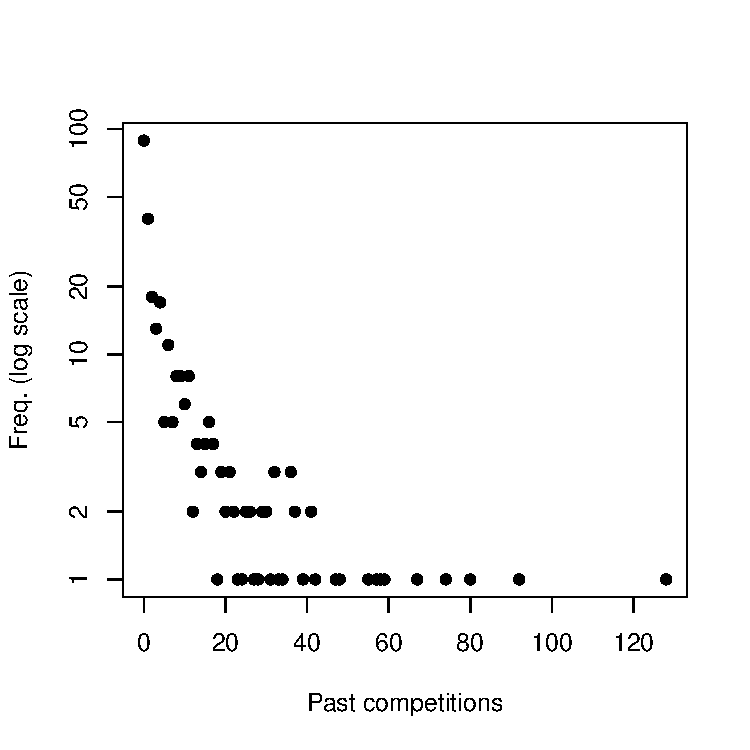
\includegraphics[width=0.45\textwidth]{%
  /Users/andrea/Documents/NTL/races/Workspace/Assets/Figures/experience-1.pdf}
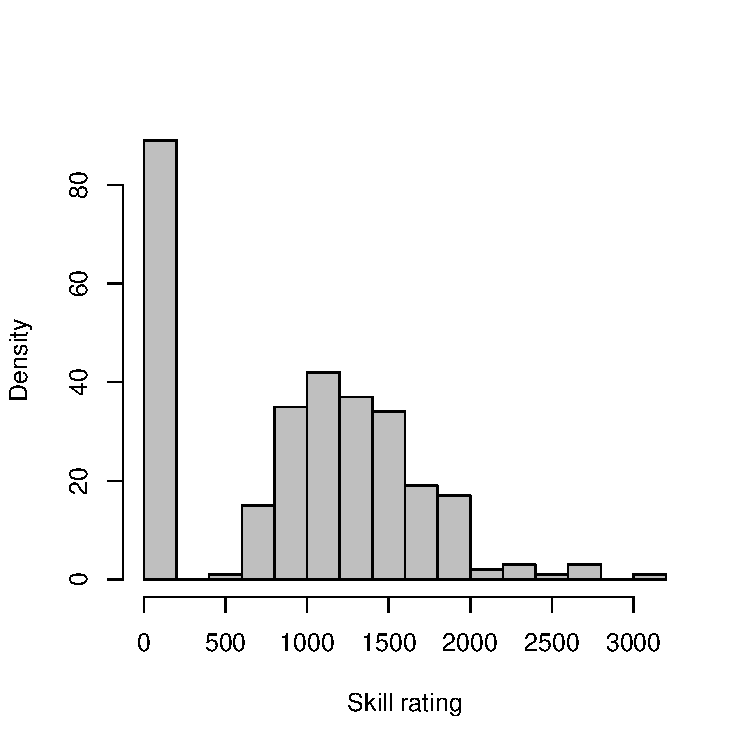
\includegraphics[width=0.45\textwidth]{%
  /Users/andrea/Documents/NTL/races/Workspace/Assets/Figures/rating-1.pdf}
\caption{Distribution of the count of past contests (left panel) and the skill ratings (right panel) of the signed-up competitors.}
\label{eq: distribution experience}
\end{figure}

\section{Empirical analysis}\label{empirical-analysis}

\subsection{Estimation results}\label{estimation-results}

Participation to the competition by treatment is shown in Figure
\ref{fig:entry}. Participation here is measured by the proportion of
registered participants per treatment who made any submission during the
eight-day submission period. Recall that competitors may decide to enter
into the competition and work on the problem without necessarily
submitting. In a tournament, for example, competitors are awarded a
prize based on their last submission and may decide to drop out without
submitting anything. However, this scenario seems unlikely. In fact,
competitors often end up making multiple submissions because by doing so
they obtain intermediate feedback via preliminary scoring (see Section
XXX for details). In a race, competitors have even stronger incentives
to make early submissions as any submission that hits the target first
wins.

\begin{verbatim}
Table xxx
\end{verbatim}

We find that the propensity to make a submission is higher in the
Tournament than in the Race and in the Tournament with reserve, but the
difference is not statistically significant (a Fisher's exact test gives
a p-value of \texttt{r\ round(fisher.test(nsub.tab)\$p.val,3)}). As
discussed in Section XXX, we may not have enough power to detect
differences below 5 percentage points. However, we find the same
not-significant result in a parametric regression analysis of treatment
differences with controls for the demographics and past experience on
the platform; see Table \ref{entry}. Adding individual covariates
reduces variability of outcomes, potentially increasing the power of our
test. In particular, Table \ref{entry} reports the results from a
logistic regression on the probability of making a submissions. Column 1
reports the results from a baseline model with only treatment dummies.
Column 2 adds demographics controls, such as the age, education, and
gender. Column 3 adds controls for the past experience on the platform.
Across all these specifications, the impact of the treatment dummies
(including room size) on entry is not statistically significant.

\subsection{Simulation results}\label{simulation-results}



  
% Bibliography
\newpage
\singlespacing
\bibliography{refs}
\end{document}
